%eita \usetikzlibrary{shapes.geometric, arrows, positioning} er pore paste korbi
%Quote package define
\usepackage{framed}
\definecolor{shadecolor}{RGB}{240,240,240}
\newenvironment{magquote}
  {\begin{shaded*}\itshape\small}
  {\end{shaded*}}

% Eita direct paste korbi jayga moto
%Article 8
\article{\centering{No Matter How Fast You Run, You Can't Escape Reality}}{Md. Asif Khan}{June 28, 2025}

\begin{figure}[h!]
  \centering
  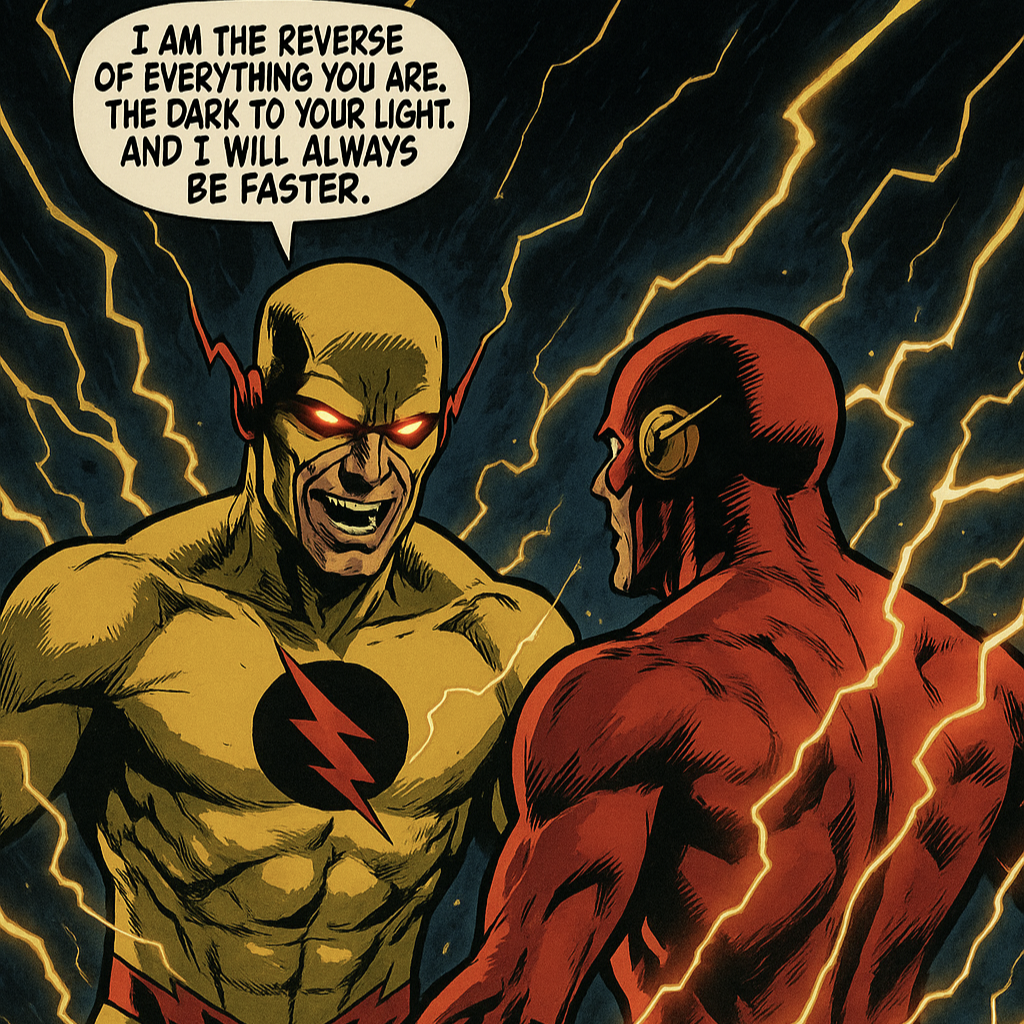
\includegraphics[width=0.9\linewidth]{reverse_.png}
  \caption*{\textit{“I am the Reverse of everything you are. The dark to your light. And I will always be faster.” — Eobard Thawne to Barry Allen}}
\end{figure}

\subsection*{Introduction}
In Detective Comics, few rivalries are as intense as the one between \textbf{Barry Allen},the Flash and \textbf{Eobard Thawne },the Reverse-Flash. It is a conflict not only of just speed but also of philosophy, trauma, and time itself. Their enmity forms a cosmic ouroboros—an eternal chase where the hunter and hunted are forever in loops of fate and obsession.

This is more than a superhero-villain feud. It’s a story of love twisted into hatred, of admiration turned into madness, and of a hero whose very existence cursed him with his deadliestenemy.


\subsection*{Barry Allen: The Fastest Human Alive}
Introduced in \textit{Showcase \#4} (1956), Barry Allen redefined the Golden Age Flash for the modern era. A forensic scientist gifted with super-speed via a lightning strike and chemical spill, Barry channels his trauma (notably the death of his mother and the wrongful imprisonment of his father) into a mission to protect Central City as \textit{The Flash}.

\subsection*{Eobard Thawne: The Twisted Fan}
Hailing from the 25th century, Eobard Thawne was once \textit{The Flash’s biggest admirer}. He discovered the Speed Force and sought to recreate Barry’s powers. Upon doing so, he idolized the Flash---until he traveled back in time and learned his destiny: to become Barry’s greatest enemy.

Thawne’s admiration became bitterness when he discovered that in his future, he was destined not to be loved like the Flash, but hated and feared. His attempts to be like Barry only isolated him further. His envy turned to wrath, and he swore not only to defeat Barry but to unravel his life, piece by piece.

From that realization, the \textit{Reverse-Flash} was born not just from hate, but also from obsession. In \textit{The Flash: Rebirth} (2009) by Geoff Johns, Thawne even creates his own \textbf{Negative Speed Force}, corrupting the very energy that empowers speedsters.

\begin{figure}[h!]
  \centering
  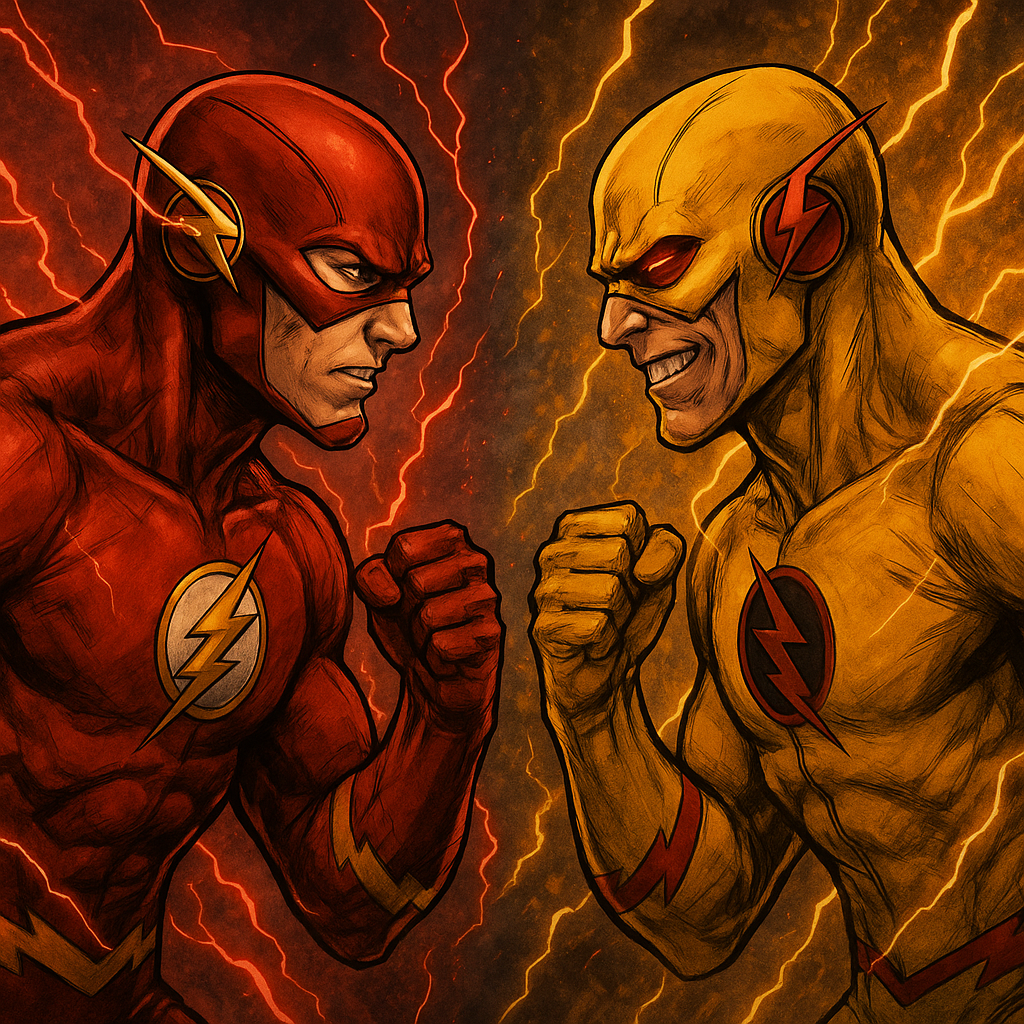
\includegraphics[width=0.9\linewidth]{vs.png}
  \caption*{\textit{Two sides of the Speed Force: Flash and Reverse-Flash}}
\end{figure}

In the CW's \textit{The Flash} television series, Thawne’s story is further expanded. After traveling back in time and being stranded in the 21st century, Thawne murders Dr. Harrison Wells and takes his identity. Under the alias of Wells, he becomes the founder of S.T.A.R. Labs and mentors Barry Allen. Using his future knowledge, he orchestrates the particle accelerator explosion, which ultimately gives Barry his powers. Ironically, the man who would become the Flash is created by his own worst enemy.

\subsection*{Time’s Cruel Loop: Their Twisted Conflict}
The defining moment of their rivalry occurs in \textit{The Flash (Vol. 2) \#197} and \textit{Flashpoint} (2011): \textbf{Thawne murders Barry’s mother}, Nora Allen, to make Barry suffer. In the aftermath, Barry’s father, \textbf{Henry Allen}, is wrongly convicted of the murder and sentenced to prison—despite his innocence. This single act not only traumatizes young Barry but also shapes his future path: he becomes a forensic scientist to uncover the truth and clear his father's name.

\begin{figure}[h!]
  \centering
  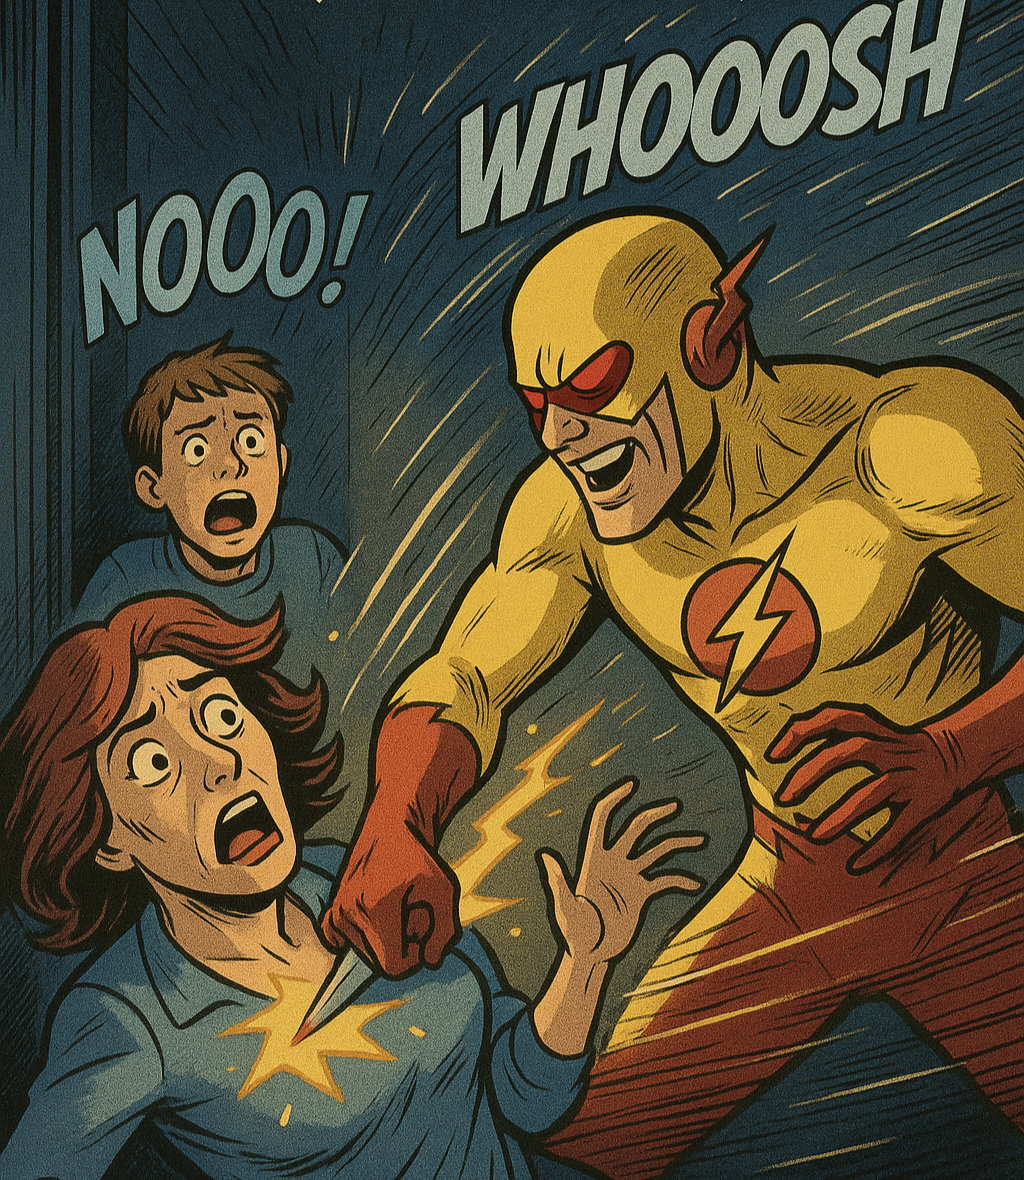
\includegraphics[width=0.9\linewidth]{flashmomdead.png}
  \caption*{\textit{Nora Allen’s death: the event that turned a child into The Flash.}}
\end{figure}

This tragedy reshapes Barry’s entire life and sets off the time-bending saga that would eventually birth the \textit{Flashpoint} universe.

In \textit{Flashpoint}, Barry attempts to undo his mother's death, but his interference leads to a fractured, dystopian timeline. Ironically, Thawne reveals that Barry was the one who created the chaos---not him.

\begin{magquote}
“Every hero needs an origin story. I just made yours the worst one imaginable.”
\hfill --- Eobard Thawne
\end{magquote}

\subsection*{Themes: Obsession, Identity, and Destiny}
\begin{magquote}
“You know what the greatest tragedy is, Barry? It’s not that I killed your mother. It’s that you were too slow to stop me.”  
\hfill --- Eobard Thawne, \textit{CW's The Flash}
\end{magquote}

The Flash and Reverse-Flash are two sides of the same coin. Barry represents \textbf{hope, justice, and legacy}, while Thawne stands for \textbf{vengeance, corruption, and obsession}.

Their battles are more than just physical races---they are existential struggles:
\begin{itemize}
  \item \textbf{Free Will vs. Determinism}: Barry constantly fights to change destiny, while Thawne ensures it remains a loop.
  \item \textbf{Heroism vs. Narcissism}: Barry sacrifices for others; Thawne is driven by ego and a need for recognition.
\end{itemize}

This theme of self-obsession versus self-sacrifice extends to other speedster enemies, such as \textbf{Savitar}. In both the comics and the CW series, Savitar is portrayed as a distorted, godlike speedster obsessed with power and control. In the show, Savitar is revealed to be a time remnant of Barry Allen himself---a future version consumed by pain and rejection, turned villainous in a desperate bid for relevance. Savitar adds another layer to the Flash's struggles: sometimes the darkest enemy is the one created by your own mistakes.

\subsection*{The Impact on the DC Universe}
In \textit{Flashpoint}, Thawne’s manipulation reshapes the entire DC Universe, leading to the \textit{New 52} reboot. Thawne’s hatred is so profound that he returns from death repeatedly---through time manipulation, clones, Speed Force resurrection, and paradoxes.

\subsection*{The Paradox of Hate}
\begin{magquote}
“You created me, Barry. Just like I created you. We’re echoes in a loop we can never outrun.”  
\hfill --- Eobard Thawne
\end{magquote}

The ultimate irony? \textbf{Thawne only exists because of Barry Allen.} Without the Flash, there is no Reverse-Flash. But without the trauma Thawne caused, Barry wouldn’t become the man he is.

It’s a loop. A tragic, cruel loop.

And no matter how many timelines Barry tries to fix, Thawne always finds a way to return---faster, meaner, more obsessed.

\subsection*{Conclusion: No Finish Line}
\begin{magquote}
“The truth is, we are forever bound---past and future, hate and hope.”  
\hfill --- Barry Allen, \textit{The Flash (Vol. 3) \#9}
\end{magquote}

The war between Flash and Reverse-Flash isn’t just a superhero clash---it’s a metaphor. For how our past shapes us. For how light attracts darkness. And for how even the fastest man alive can’t outrun the scars of destiny.

In the end, the chase continues. Not just in comics---but in the very heartbeat of DC’s legacy.

\subsection*{References}
\begin{itemize}
  \item \textit{Showcase \#4} (1956) – Debut of Barry Allen as The Flash.
  \item \textit{The Flash: Rebirth} (2009) – Origin of Reverse-Flash's Negative Speed Force.
  \item \textit{The Flash (Vol. 2) \#197} – Reveals Thawne killed Barry’s mother.
  \item \textit{Flashpoint} (2011) – Major alternate timeline caused by Barry trying to save his mother.
  \item \textit{The Flash (Vol. 5) \#50} – Psychological confrontation between Barry and Thawne.
  \item \textit{CW's The Flash} (2014–present) – TV portrayal of their enmity and Savitar arc.
  \item \textit{DC Rebirth \#1} (2016) – Hints at ongoing consequences of their conflict.
\end{itemize}

\clearpage
\cleardoublepage
